\documentclass[12pt, french]{article}

\usepackage{fancyhdr, fancybox, lastpage, makecell,amssymb}
\usepackage[most]{tcolorbox}
\usepackage[a4paper, margin={0.3in, .75in}]{geometry}
\usepackage{wrapfig}
\pagestyle{fancy}
\renewcommand\headrulewidth{1pt}
\renewcommand\footrulewidth{1pt}
\fancyhf{}
\rhead{ \em{Zakaria Haouzan}}
\lhead[C]{\em{2ème année baccalauréat SM-X}}
\chead[C]{}
\rfoot[C]{\emph{Propagation d’une onde lumineuse}}
\lfoot[R]{ \emph{Exercices Supplémentaires}}
\cfoot[]{\em{Page \thepage / \pageref{LastPage}}}


\newtcolorbox{Box2}[2][]{
                lower separated=false,
                colback=white,
colframe=white!20!black,fonttitle=\bfseries,
colbacktitle=white!30!gray,
coltitle=black,
enhanced,
attach boxed title to top left={yshift=-0.1in,xshift=0.15in},
title=#2,#1}


\begin{document}
\begin{center}
   \shadowbox {\bf{Propagation d’une onde lumineuse}}
\end{center}

\vspace{-0.2cm}
%%_________________________Exercice ! :"_________________________Exercice
%   \begin{center}
	   %\vspace{-0.6cm}
	%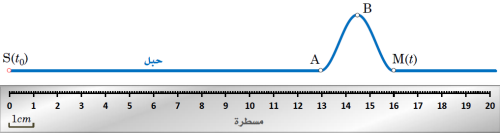
\includegraphics[width=0.6\textwidth ]{./img/Exercice01.png}
  %\end{center}



\begin{Box2}{\textbf{Exercice 1 : Propagation d’une onde lumineuse }}

	\textbf{ Partie 1 : Détermination du diamètre d’un fil de pêche :}

	\emph{ Le fil de pèche est fabrique à partir du nylon qui supporte une grande résistance au poisson pèche, son diamètre est très petit pour ne pas être vue par les poissons.}
\\Pour déterminer le diamètre a d’un fil de pêche, on l’éclaire à l’aide d’une
 source laser de longueur d’onde $\lambda$, sur un écran situe à une distance D du fil
on obtient des taches lumineuses, la largeur de la tache centrale est L. (voir figure)

\textbf{Les données : $\lambda=623,8nm$ \hspace{1cm} D=3m \hspace{1cm} L=7,5cm}

\textbf{1- }Donner le nom du phénomène observe sur la figure

\textbf{2- }Sachant que l’écart angulaire $\theta$ entre le milieu de la tache centrale et l’une de ces extrémités est $\theta = \frac{\lambda}{a}$, Trouver la valeur de a en fonction de D, L et $\lambda$ dans le cas ou $\theta$ est petite. \textbf{calculer la valeur de a.}

\textbf{3- }On remplace le laser par un autre de longueur d’onde $\lambda'$ et on obtient une tache centrale de largeur $L'=8cm$. \textbf{Exprimer $\lambda'$ en fonction de $\lambda$, L et $L'$, calculer $\lambda'$
}

\vspace{0.5cm}

\textbf{ partie 2 : la longueur d’onde d’une onde lumineuse dans le verre :}

Une source laze envoie un faisceau lumineux monochromatique sur la face d’un prisme de verre
d’indice de réfraction n=1,58

Les données :

\begin{itemize}
	\item La longueur d’onde du faisceau lumineux : $\lambda_0=665,4nm$.

	\item La vitesse de propagation de la lumière dans le vide et l’air : $c=3.10^8m/s^2$.
\end{itemize}

\textbf{1- }Calculer la vitesse v de propagation du faisceau lumineux dans le prisme.

\textbf{2- }Trouver la valeur de la longueur d’onde $\lambda_1$ des faisceaux lumineux dans le prisme.

\end{Box2}
%%_________________________Exercice !2 :"_________________________Exercice
\begin{Box2}{Exercice 2 :Les fibres optiques  }

	\emph{Les fibres optiques permettent la transmission d’informations numériques avec des vitesses très
grandes et à haut débits en comparaison avec d’autres milieux.
Pour déterminer l’indice de réfraction du milieu transparent constituant le cœur d’une fibre optique,
on a réalisé un dispositif expérimental représenté sue la figure 1, où les récepteurs R1 et R2 permettent
de transformer l’onde lumineuse monochromatique issue de la source laser, en tension électrique qu’on
affiche sur l’écran d’un oscilloscope comme indiqué sur la figure 2.}

Sensibilité horizontale : $S_H = 0,2 \mu{s}.div^{-1}$

Célérité de propagation de la lumière dans le vide : $c = 3.10^8 m/s$ 

\textbf{1- }Calculer le retard temporel $\tau$ enregistré entre $R_1$ et $R_2$.

\textbf{2- }Sachant que la célérité de propagation de l’onde lumineuse à l’intérieur du cœur de la fibre
optique est $v = 1,87.10^8 m/s$, déduire l’indice de réfraction n du milieu transparent constituant
le cœur d’une fibre optique.
  \begin{center}
	  %\vspace{-0.6cm}
	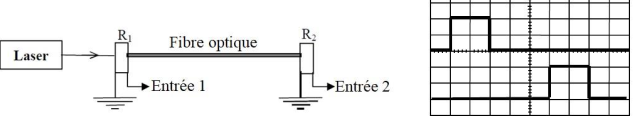
\includegraphics[width=0.8\textwidth]{./img/ex2.png}
  \end{center}

\end{Box2}

\begin{Box2}{Exercice 3 :fibres optique et indice de réfraction}
	\emph{Pour déterminer l’indice de réfraction du milieu transparent constituant le cœur d’une fibre
optique, on a réalisé un dispositif expérimental représenté sue la figure 1, où les récepteurs R1 et R2
permettent de transformer l’onde lumineuse monochromatique issue de la source laser, en tension
électrique qu’on affiche sur l’écran d’un oscilloscope comme indiqué sur la figure 2.}
  \begin{center}
	  %\vspace{-0.6cm}
	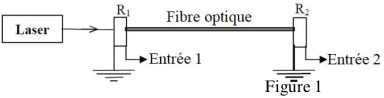
\includegraphics[width=0.44\textwidth]{./img/ex3_1.png}
	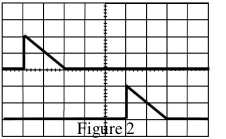
\includegraphics[width=0.26\textwidth]{./img/ex3_2.png}

  \end{center}

  On donne :  -Sensibilité horizontale : $S_H = 0,2 \mu{s}/div$

  Sur l’étiquette du laser on lit, la longueur d’onde dans le vide : $\lambda_0 = 600 nm$ .
Pour déterminer la vitesse d’une onde lumineuse dans une fibre optique de longueur $L = 200 m$, on
a réalisé le montage de la figure 1, où $R_1$ et $R_2$ des capteurs permettant de transformer le signal
lumineux en signal électrique qu’on affiche sur l’écran d’un oscilloscope (Figure 1)

\textbf{1- }Déterminer le retard temporel $\tau$ enregistré entre R1 et R2.

\textbf{2- }Calculer la célérité de propagation de l’onde lumineuse à l’intérieur du cœur de la fibre
optique.

\textbf{3- }Déduire la valeur de l’indice de réfraction n de la matière constituant le cœur de la fibre
optique.

\textbf{4- }Calculer la valeur de la longueur d’onde $\lambda$ à l’intérieur du cœur de la fibre optique.

\textbf{5- }Le cœur de la fibre optique est un milieu transparent dont l’indice de réfraction varie avec la
longueur de l’onde incidente selon la loi : $$n= 1,484 + \frac{5,6.10^{-15}}{\lambda^2}$$

On remplace la source lumineuse par une autre source monochromatique de longueur d’onde
dans le vide $\lambda_0' = 400 nm$, sans aucune modification dans le dispositif expérimental précédent.
Trouver la valeur du retard temporel $\tau'$ observé sur l’écran de l’oscilloscope.

\end{Box2}

\begin{tcolorbox}
	Exercice 4 : Tsunami
\end{tcolorbox}

On modélise un tsunami par une onde mécanique progressive périodique, se propageant à la
surface de l’eau avec une vitesse v variant avec la profondeur h de l’océan selon la relation $V$=$\sqrt{g.h}$
dans le cas des petites profondeurs comparées à la longueur d’onde $(\lambda >> h)$ où : $\lambda$ est la longueur
d’onde et g l’intensité de pesanteur. $g = 10m/s^2$

On étudiera la propagation d’un tsunami dans une région de l’océan de profondeur supposée\\constante: $h$ = $6000 m$.

\textbf{1- }Justifier que les ondes se propageant à la surface de l’océan sont transversales.

\textbf{2- }Calculer la vitesse de propagation des ondes dans cette région de l’océan.

\textbf{3- }Sachant que la durée séparant deux crêtes consécutives est $T = 18 min$. déterminer la valeur de
la longueur d’onde $\lambda$.

\textbf{4- }Dans le cas $(\lambda >> h)$, la fréquence des ondes tsunami reste constante lors de sa propagation vers la côte. Comment varie la longueur d’onde $\lambda$ en s’approchant de la côte ? Justifier.

\begin{wrapfigure}[6]{r}{0.26\textwidth}
  \begin{center}
	  \vspace{-0.7cm}
	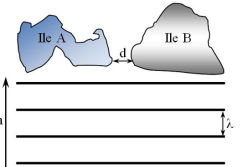
\includegraphics[width=0.26\textwidth]{./img/ex4.png}
  \end{center}
\end{wrapfigure}


\textbf{5- }L’onde tsunami passe entre deux iles A et B séparées par un détroit de largeur $d = 100 km$. On
suppose que la profondeur de l’océan aux voisinages des deux iles reste constante, et que l’onde tsunami incidente est rectiligne de
longueur d’onde $\lambda = 120 km$. (Figure ci-contre)

\textbf{5.1- }La condition pour que l’onde soit diffractée à la traversée du détroit, est-elle réalisée. Justifier.

\textbf{5.2- }Dans le cas où se produit une diffraction : Donner, en justifiant, la longueur d’onde de l’onde
diffractée. Calculer l’angle de diffraction $\theta$.

\begin{Box2}{Exercice 5 :}
	Données : La vitesse de propagation d’une onde lumineuse dans l’air est approximativement égale à
sa vitesse de propagation dans le vide $c = 3,00.108 m/s$.

\begin{wrapfigure}[2]{r}{0.26\textwidth}
  \begin{center}
	  \vspace{-1.5cm}
	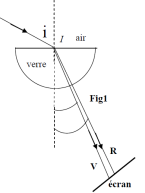
\includegraphics[width=0.26\textwidth]{./img/ex5_1.png}
  \end{center}
\end{wrapfigure}


\vspace{0.5cm}
%\begin{center}
\begin{tabular}{ |c|c|c| } 
 \hline
 Couleur de la radiation & Rouge(R) & Violet(V) \\\hline
 La longueur d’onde dans l’air en $(\mu{m})$ & 0,768 & 0,434 \\\hline 
 L’indice de réfraction du verre & 1,51 & 1,52 \\\hline 
 \hline
\end{tabular}
%\end{center}
\vspace{0.5cm}

\textbf{1 - Dispersion de la lumière :}

Un faisceau parallèle de lumière blanche arrive au point I de la surface d’un demi-
disque en verre, on observe sur l’écran (fig1) les sept couleurs du spectre allant
du rouge (R) au viole (V).

\textbf{1.1- }Exprimer la longueur d’onde $\lambda_R$ de la radiation rouge dans le verre en
fonction de l’indice de réfraction $n_R$ du verre et de $\lambda_R0$. (longueur d’onde dans l’air de ce rayonnement).

\textbf{1.2- } L’indice de réfraction n d’un milieu transparent pour une radiation
monochromatique de longueur d’onde $\lambda_0$ dans l’air est modélisé par la
relation : $$n = A + \frac{B}{\lambda^2_0} $$
dont A et B sont des constantes qui dépondent du milieu. Calculer la valeur de A et celle de B pour le verre utilisé.

\textbf{2 - Diffraction de la lumière :}

On réalise l’expérience de la diffraction d’une lumière monochromatique de longueur d’onde $\lambda$
dans l’air émise par un dispositif laser, en utilisant une fente de largeur a comme l’indique la figure
2. On mesure la largeur d de la tache centrale pour différentes valeurs de la largeur a de la fente et on
représente graphiquement $d = f(\frac{1}{a})$ , on obtient alors la courbe indiquée dans la figure 3.

\textbf{2.1- }Trouver l’expression de d en fonction de $\lambda$, a et D.

\textbf{2.2- }A l’aide de la fig 3, déterminer la valeur de $\lambda$.

\begin{center}
	  \vspace{-1.5cm}
	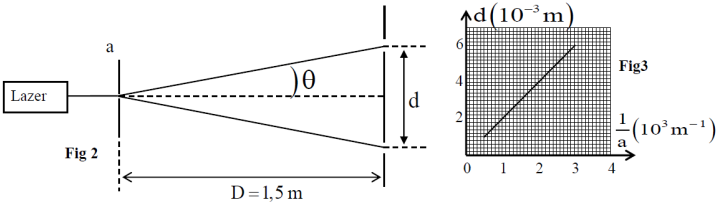
\includegraphics[width=0.9\textwidth]{./img/ex5_2.png}
  \end{center}
\end{Box2}


%\begin{wrapfigure}[6]{r}{0.36\textwidth}
  %\begin{center}
	  %\vspace{-0.6cm}
	%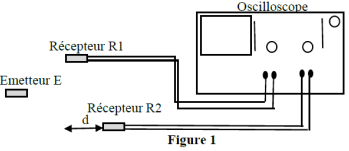
\includegraphics[width=0.36\textwidth]{./img/ex2_1.png}
  %\end{center}
%\end{wrapfigure}

	  %\vspace{-1cm}
	%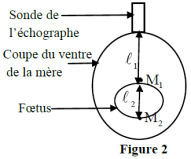
\includegraphics[width=0.26\textwidth]{./img/ex2_2.png}
  %\end{center}
%\end{wrapfigure}


%\begin{wrapfigure}{r}{0.22\textwidth}
  %\begin{center}
	  %\vspace{-0.6cm}
	%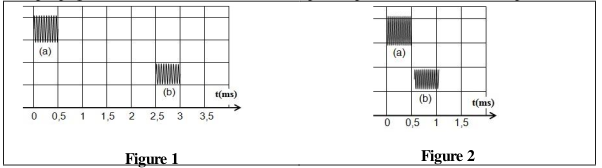
\includegraphics[width=0.22\textwidth]{./img/Ex2.png}
  %\end{center}
%\end{wrapfigure}
%\vspace{2cm}
%\begin{center}
   %\Large{ \em{Exercices Supplémentaires}}
%\end{center}


%\vspace{-0.7cm}
%%_________________________Exercice 5 : _________________________Exercice
%\begin{Box2}{Exercice 5 :Les ondes sonores }
%4
%\end{Box2}
%%_________________________Exercice 6 : _________________________Exercice
%\begin{Box2}{Exercice 6 : échographie}
%6
%\end{Box2}

\end{document}
